% !TeX root=main.tex
\faculty{پردیس دانشکده‌های فنی}
\department{دانشکده مهندسی برق و کامپیوتر}
\subject{مهندسی برق}
\field{شبکه‌های مخابراتی}

\title{سكوی اینترنت اشیاء مجازی جهت كاربرد شهر هوشمند}
\firstsupervisor{دکتر وحید شاه منصوری}
%\secondsupervisor{استاد راهنمای دوم}
%\firstadvisor{استاد مشاور اول}
%\secondadvisor{استاد مشاور دوم}
\name{علی}
\surname{سرورامینی}
\studentID{۸۱۰۱۹۵۲۵۲}
\thesisdate{شهریور ۱۳۹۸}
%\projectLabel{پایان‌نامه}
%\degree{}

\firstPage

\cleartorightpage
\besmPage

\cleartorightpage
\firstPage

\cleartorightpage
% \newpage

% \thispagestyle{empty}

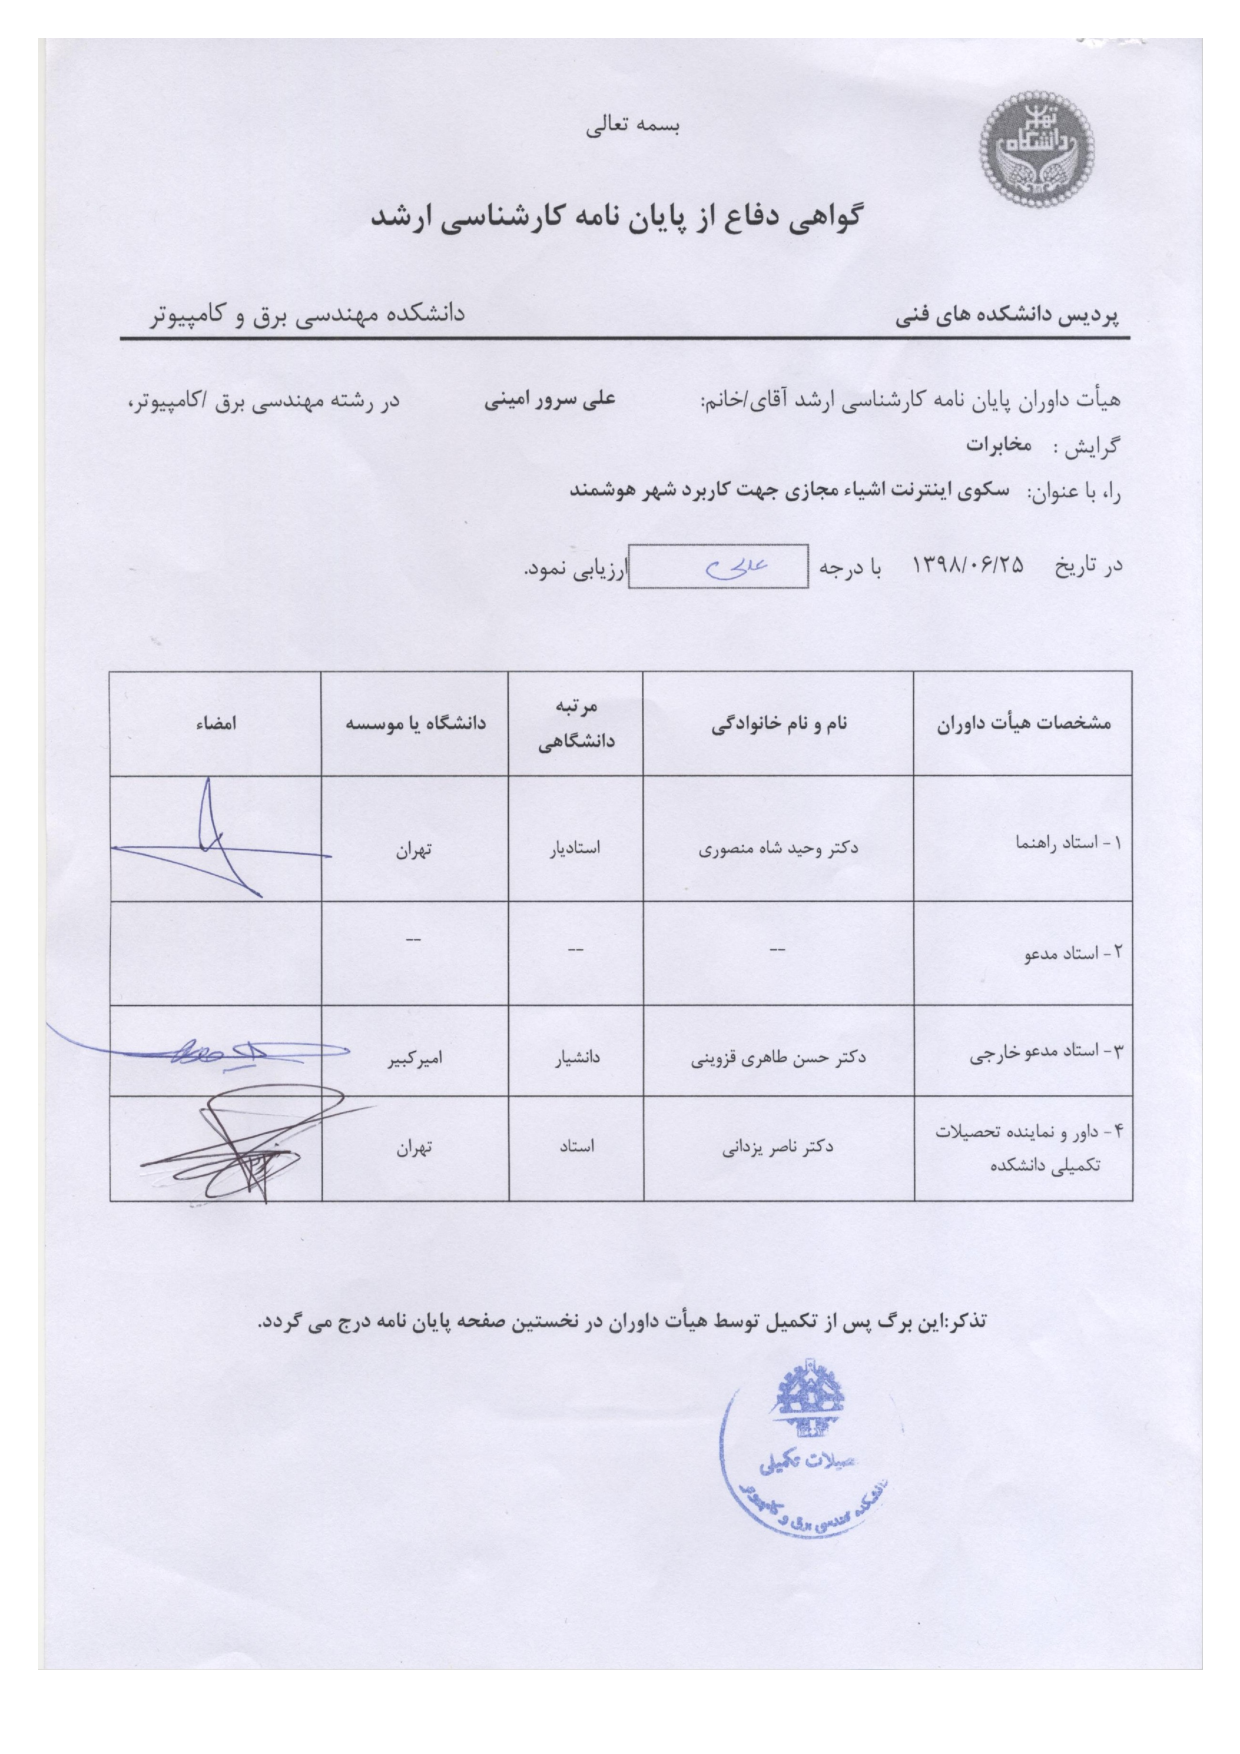
\includepdf{graphics/cert}
% \setcounter{page}{1}
% \vspace{-15cm}
% \begin{center}
%   \vspace{-5cm}
  
%   \makebox[\textwidth]{\vspace{-5cm}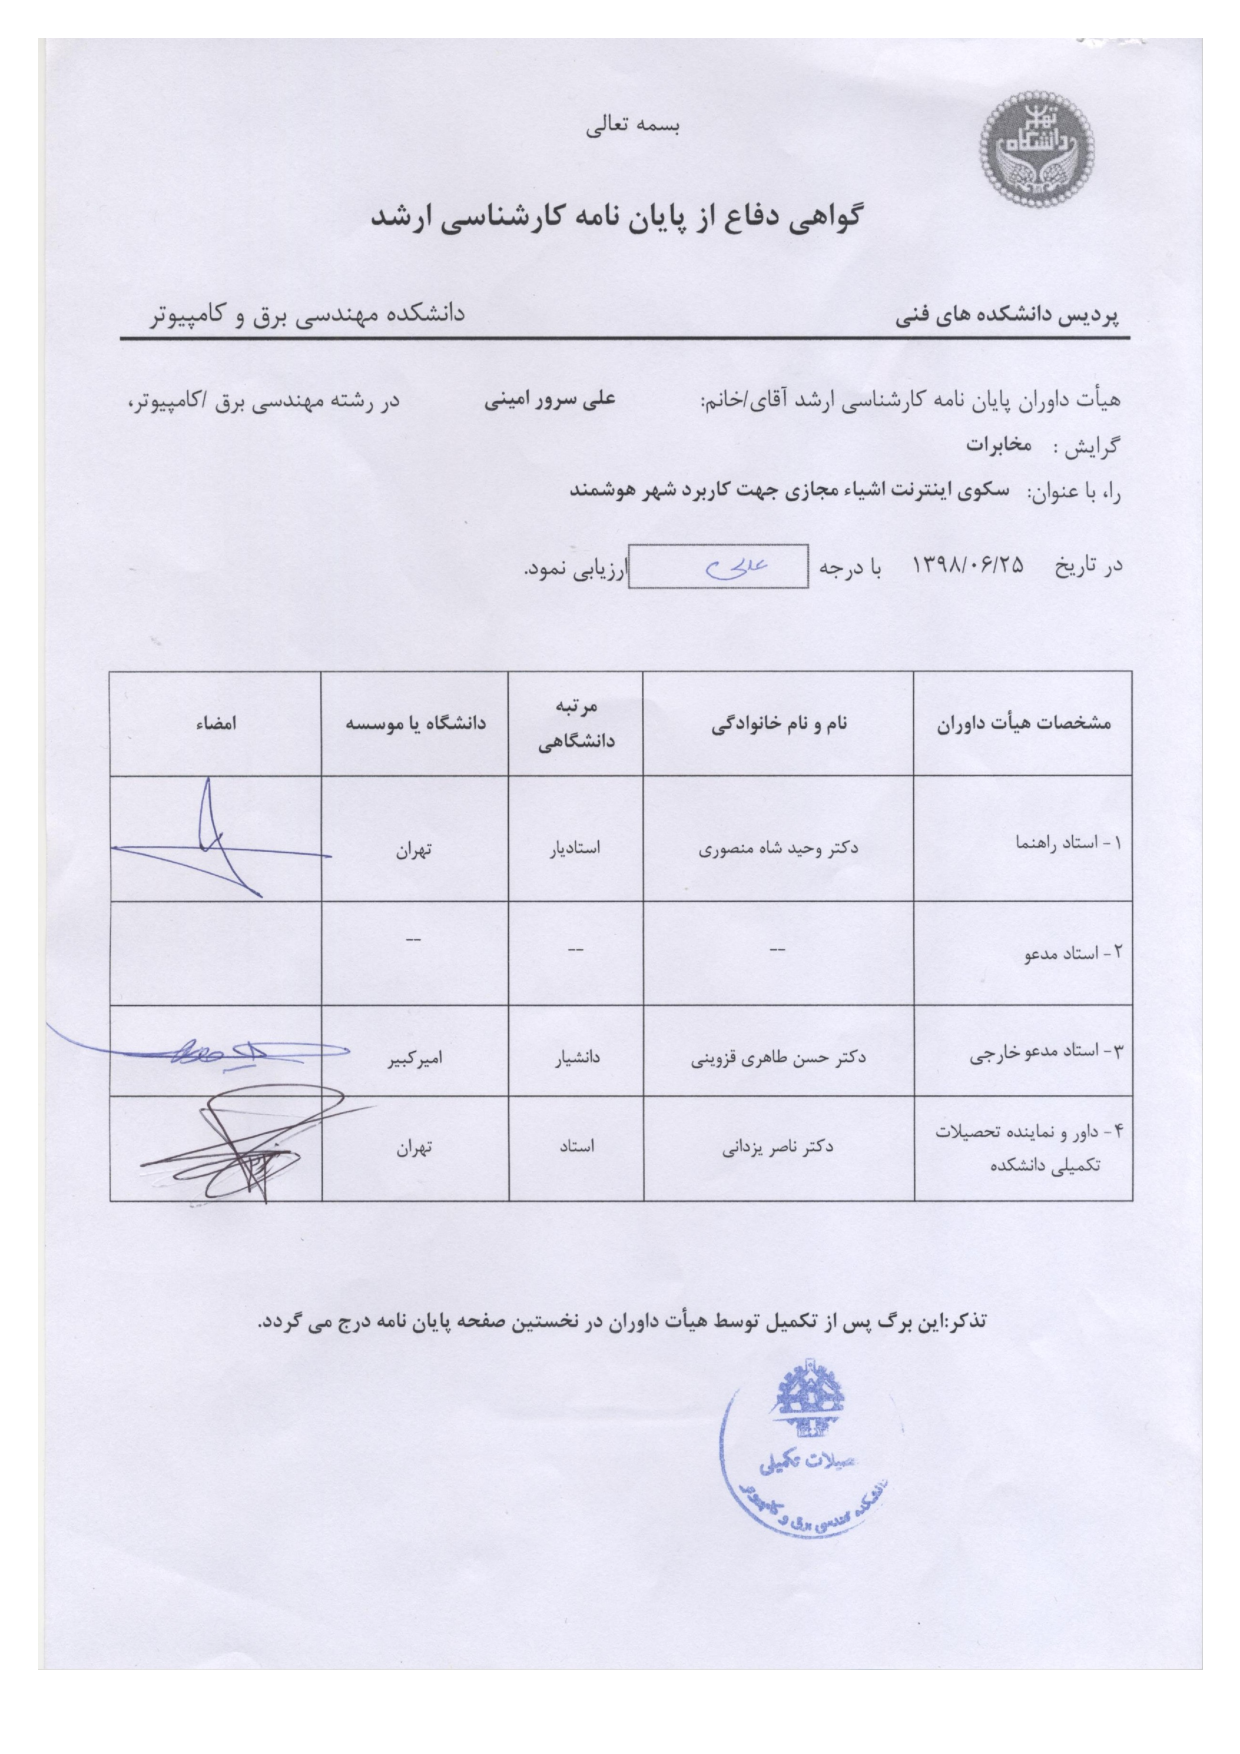
\includegraphics[width=\paperwidth]{graphics/cert}}
% \end{center}

% \incgraph[width=\paperwidth]{graphics/cert}

% \davaranPage
%\vspace{.5cm}
% در این قسمت اسامی اساتید راهنما، مشاور و داور باید به صورت دستی وارد شوند
%\renewcommand{\arraystretch}{1.2}
% \begin{center}
%   \begin{tabular}{|c|p{30mm}|c|c|p{25mm}|c|}
%     \hline
%     ردیف	  & سمت                                           & نام و نام خانوادگی    & مرتبه \newline دانشگاهی &	دانشگاه یا مؤسسه               & امضـــــــــــــا \\
%     \hline
%     ۱       & استاد راهنما                                  & دکتر وحید شاه‌منصوری   & استاد‌یار                & دانشگاه تهران                   &                   \\
%     \hline
%     ۲       &‌ استاد مدعو خارجی                              & دکتر حسن طاهری قزوینی & دانشیار                 & دانشگاه \newline صنعتی امیرکبیر &                    \\
%     \hline
%     ۳       & داور و نماینده \newline تحصیلات تکمیلی دانشکده & دکتر ناصر یزدانی      & استاد                   & دانشگاه تهران                   &                    \\
%     \hline
%   \end{tabular}
% \end{center}

\cleartorightpage
\esalatPage

\cleartorightpage
\thispagestyle{empty}
{\Large تقدیم به:} \\
\begin{flushleft}
  {
    \huge
    پدر و مادرم
  }
\end{flushleft}

\cleartorightpage
\begin{acknowledgementpage}
  سپاس خداوندگار حکیم را که با لطف بی‌کران خود، آدمی را زیور عقل آراست.

  در آغاز وظیفه‌ خود می‌دانم از زحمات بی‌دریغ استاد راهنمای خود، جناب آقای دکتر وحید شاه‌منصوری، صمیمانه تشکر و قدردانی کنم که قطعاً بدون راهنمایی‌های ارزنده‌ ایشان، این مجموعه به انجام نمی‌رسید.

  در پایان، بوسه می‌زنم بر دستان خداوندگاران مهر و مهربانی، پدر و مادر عزیزم و بعد از خدا، ستایش می‌کنم وجود مقدس‌شان را و تشکر می‌کنم از خانواده عزیزم به پاس عاطفه سرشار و گرمای امیدبخش وجودشان، که بهترین پشتیبان من بودند.
% با استفاده از دستور زیر، امضای شما، به طور خودکار، درج می‌شود.
\signature
\end{acknowledgementpage}

\keywords{اینترنت اشیاء، شهر هوشمند، پردازش لبه، تخصیص منابع}
\fa-abstract{
  با حرکت به سمت عصر اینترنت اشیاء، تعداد دستگاه‌های متصل به اینترنت به صورت نمایی در حال افزایش است.
  تعداد زیاد دستگاه‌های متصل باعث ایجاد گلوگاه‌هایی در حوزه‌های مختلف مانند اتصال دستگاه‌ها و انتقال و پردازش داده‌ها می‌شود.
  پردازش لبه که یک الگوی پردازشی است و هدف آن پردازش داده‌ها در لبه شبکه می‌باشد، یک روش مناسب برای پردازش حجم زیاد داده‌های تولید شده توسط اشیاء متصل به اینترنت به شمار می‌رود.
  به لطف پیشرفت‌های ایجاد شده در فناوری‌های مجازی سازی، دروازه‌های شبکه و دستگاه‌های لبه شبکه می‌توانند ظرفیت پردازشی اضافی خود را در اختیار سرویس‌های اینترنت اشیاء قرار دهند.
  با این کار پردازش‌ مورد نیاز سرویس‌های اینترنت اشیاء می‌تواند توسط دستگاه‌های لبه شبکه انجام شود و ترافیک سرویس‌های ابری و تاخیر سرویس‌ها کاهش یابد.
  تعداد بسیار زیاد دستگاه‌های لبه و سرویس‌های شبکه اینترنت اشیاء، باعث پیچیده شدن مسئله تخصیص منابع پردازشی به سرویس‌های شبکه اینترنت اشیاء می‌شود.
  در این پایان نامه، به معرفی یک سکوی اینترنت اشیاء مجازی برای استفاده در شهر هوشمند می‌پردازیم.
  این سکو وظیفه تخصیص منابع پردازشی مورد نیاز سرویس‌های اینترنت اشیاء را برای تعداد زیاد سرویس‌ها برعهده می‌گیرد.
  تخصیص منابع برای دو حالت بررسی می‌شود.
  در حالت اول تخصیص منابع در حالتی بررسی می‌شود که هر سرویس فقط می‌تواند از یک منبع پردازشی استفاده کند و هر منبع پردازشی هم می‌تواند به یک سرویس اختصاص پیدا کند.
  در حالت دوم، هر سرویس می‌تواند از چند منبع پردازشی استفاده کند و هر منبع پردازشی هم می‌تواند به چند سرویس اختصاص پیدا کند.
  در هر دو حالت، به فرمول‌بندی مسئله تخصیص منابع پردازشی برای سرویس‌های شبکه اینترنت اشیاء پرداخته می‌شود.
  مسئله به صورت یک مسئله بهینه سازی مدل می‌شود که هدف آن بیشینه کردن مجموع سود سرویس‌ها است.
  مسئله بهینه‌سازی نهایی یک مسئله برنامه‌ریزی غیرخطی عدد صحیح مخلوط می‌باشد که در حالت کلی به سختی حل می‌شود.
  الگوریتم‌های ارائه شده برای حل این مسئله جوابی قابل قبول برای آن بدست می‌دهند که به صورت توزیع شده قابل اجرا می‌باشند.
}

\cleartorightpage
\abstractPage

\cleartorightpage
